\documentclass[t, aspectratio=169]{beamer}
\usepackage{amsmath,amsfonts,amsthm,amstext,amssymb, xcolor, tikz, pgf, mathrsfs, polynom, pifont, tabto}

% ----------------------------------------------------------
% Theme Setup

% Use Metropolis Theme
\usetheme[numbering=fraction]{metropolis}
\setbeamertemplate{blocks}[rounded][shadow=false]
\makeatletter
\setlength{\metropolis@titleseparator@linewidth}{1pt}
\makeatother

% Define Colors
\definecolor{chargerblue}{HTML}{002764}
\definecolor{chargerred}{HTML}{e02034}
\definecolor{bggray}{HTML}{d0d3d4}

% Set Colors
\setbeamercolor{title}{fg=chargerblue}
\setbeamercolor{background canvas}{bg=white}
\setbeamercolor{title separator}{fg=chargerred}
\setbeamercolor{structure}{fg=chargerblue}
\setbeamercolor{frametitle}{fg=white, bg=chargerblue}
\setbeamercolor*{normal text}{fg=chargerblue}
\setbeamercolor*{block body}{bg=bggray}
\setbeamercolor*{block title}{bg=chargerblue, fg=white}
% ----------------------------------------------------------

% ----------------------------------------------------------
% Custom Definitions, Commands, Environments, etc.

% Sets of numbers
\def\R{\mathbb{R}} % The reals
\def\N{\mathbb{N}} % The naturals
\def\Z{\mathbb{Z}} % The integers
\def\Q{\mathbb{Q}} % The rationals

% Blank space
\newcommand{\blank}[1]{\underline{\hspace{#1}}} % Blank space

% Change font colors
\newcommand{\cyan}[1]{{\color{cyan}{#1}}} % Changes font to cyan
\newcommand{\red}[1]{{\color{red}{#1}}} % Changes font to red
\newcommand{\magenta}[1]{{\color{magenta}{#1}}} % Changes font to magenta
\newcommand{\orange}[1]{{\color{orange}{#1}}} % Changes font to orange
\newcommand{\yellow}[1]{{\color{yellow}{#1}}} % Changes font to yellow
\newcommand{\violet}[1]{{\color{violet}{#1}}} % Changes font to violet
\newcommand{\green}[1]{{\color{green}{#1}}} % Changes font to green
\newcommand{\blue}[1]{{\color{blue}{#1}}} % Changes font to blue
\newcommand{\white}[1]{{\color{white}{#1}}} % Changes font to white

% Fitted inclusion symbols
\newcommand{\fp}[1]{\left({#1}\right)} % Fitted parentheses around content
\newcommand{\fb}[1]{\left[{#1}\right]} % Fitted brackets
\newcommand{\lhoi}[1]{\left({#1}\right]} % Left half-open interval
\newcommand{\rhoi}[1]{\left[{#1}\right)} % Right half-open interval
\newcommand{\set}[1]{\left\{{#1}\right\}} % Fitted braces (useful for sets)
\newcommand{\av}[1]{\left|{#1}\right|} % Fitted absolute value bars

% Augmented Matrix Environment
\newenvironment{amatrix}[1]{%
	\left[\begin{array}{@{}*{#1}{c}|c@{}}
	}{%
	\end{array}\right]
}

% Miscellaneous
\def\then{\Rightarrow}
\def\to{\rightarrow}
\def\d{^{\circ}}
\newcommand{\?}{\stackrel{?}{=}}
\newcommand{\cmark}{\text{ \ding{51}}}
\newcommand{\xmark}{\text{ \ding{55}}}

% Coordinate Plane (Four-Quadrant)
\def\coordplane {
	\begin{tikzpicture}        \draw[step=0.25cm,black,very thin,opacity=0.25] (-2.5cm, -2.5cm) grid (2.5cm, 2.5cm);
		\draw[<->,thick,black] (-2.5cm, 0) -- (2.5cm, 0) node[anchor=north west,pos=0.94,font=\scriptsize]{$x$};
		\draw[<->,thick,black] (0,-2.5cm) -- (0, 2.5cm) node[anchor=south east,font=\scriptsize,pos=0.94]{$y$};
	\end{tikzpicture}
}

% Coordinate Plane (One-Quadrant)
\def\onequad {
	\begin{tikzpicture}
		\draw[step=0.25cm, black, very thin, opacity=0.25] (0,0) grid (7.5cm,5cm);
		\draw[->, thick, black] (0,0) -- (7.5cm, 0) node[anchor=north west,font=\scriptsize,pos=0.94]{$x$};
		\draw[->, black, thick] (0,0) -- (0,5cm) node[anchor=south east,font=\scriptsize,pos=0.94]{$y$};
	\end{tikzpicture}
}
% ----------------------------------------------------------

% ----------------------------------------------------------
% Presentation Information
\title[3-1]{Measures of Central Tendency}
\subtitle{Section 3-1}
\author{Jacob Ayers}
\institute{Lesson \#5}
\date{MAT 110}
% ----------------------------------------------------------

\begin{document}
	
	% Slide 1 (Title Slide)
	\begin{frame}
		\titlepage
	\end{frame}
	
	% Slide 2 (Objectives)
	\begin{frame}{Objectives}
		\begin{itemize}
			\item Find the mean of ungrouped and grouped data sets
			\item Find the median of ungrouped data sets
			\item Find the mode of ungrouped data sets, or the modal class of grouped data sets
			\item Find the midrange of ungrouped data sets
			\item Compute weighted means
		\end{itemize}
	\end{frame}

	\begin{frame}{Measures of Central Tendency}
		When you think about taking an average, what comes to mind? \pause
		
		It turns out, there are several methods of obtaining an average. \pause
		
		In this lesson, we will look at four: \begin{itemize}
			\item Mean
			\item Median
			\item Mode
			\item Midrange
		\end{itemize}
	
		We'll learn formulas for each of these, but a graphing calculator will save us time in performing the computations. \pause
		
		I will be using the TI-84 Plus in this video, but I have also made a video showing you how to use a Casio to perform the computations.
	\end{frame}

	\begin{frame}{Mean for Ungrouped Data}
		Most people associate ``average" with mean. \pause
		
		To compute the mean for an ungrouped data set, add up all the data values and divide the sum by the number of values in the data set. \pause
		
		Mathematically, $\overline{X} = \dfrac{\sum x}{n}$ represents the sample mean and $\mu = \dfrac{\sum X}{N}$ represents the population mean. \pause
		
		When computing the mean, always report the value rounded to one more place than the raw data.
	\end{frame}

	\begin{frame}{Mean for Ungrouped Data}
		The number of confirmed avian flu cases for a 9-year period is shown. Find the mean.
		
		$4 \; 46 \; 98 \; 115 \; 88 \; 44 \; 73 \; 48 \; 62$ \pause \vspace{32pt}
		
		Using a graphing calculator, we find a mean of approximately $64.2$ cases/year.
	\end{frame}

	\begin{frame}{Mean for Ungrouped Data}
		The data shows the heights in feet of 14 roller coasters. Find the mean for the data.
		
		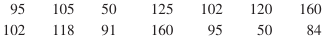
\includegraphics[width=3in]{coaster-data.png} \pause \vspace{32pt}
		
		Using a graphing calculator, we find a mean of approximately $104.1$ feet.
	\end{frame}

	\begin{frame}{Mean for Grouped Data}
		To find the mean for grouped data, we assume that the mean of all the raw data values in each class is equal to the midpoint of the class. \pause
		
		This assumption is not necessarily true, but it is the best method of estimating the mean given that we don't have the raw data to work with. \pause
		
		The formula for the mean for a grouped data set is $\overline{X} = \dfrac{\sum (f \cdot X_m)}{n}$ (see p. 113 for more information).
		
		Graphing calculators can also compute means for grouped data.
	\end{frame}

	\begin{frame}{Mean for Grouped Data}
		The data shows the number of points the winning team scored in the Rose Bowl. Find the mean of the data. \pause
		
		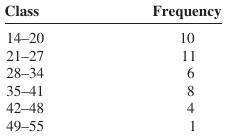
\includegraphics[width=1.5in]{rose-data.png} \pause
		
		First, find the midpoints of each class (you should verify): $17, 24, 31, 38, 45, 51$ \pause \vspace{32pt}
		
		Using a graphing calculator, we find a mean of $28.9$ points.
	\end{frame}

	\begin{frame}{Mean for Grouped Data}
		Here is the hand computation for the previous example:
		
		$\begin{tabular}{|c|c|c|c|} \hline
			Class & Midpoint & Frequency & $f \cdot X_m$ \\ \hline
			14-20 & 17 & 10 & 170 \\ \hline
			21-27 & 24 & 11 & 264 \\ \hline
			28-34 & 31 & 6 & 186 \\ \hline
			35-41 & 38 & 8 & 304 \\ \hline
			42-48 & 45 & 4 & 180 \\ \hline
			49-55 & 52 & 1 & 52 \\ \hline
			TOTALS &  & 40 & 1156 \\ \hline
		\end{tabular}$ \pause
	
		Thus, the mean is $\dfrac{1156}{40} = 28.9$.
	\end{frame}

	\begin{frame}{Median}
		The \textit{median} is the midpoint of the data set. \pause
		
		To find the median of a data set by hand: \begin{enumerate}[1)]
			\item Sort the data from least to greatest \pause
			\item Find the middle values (by crossing out outer values until there are 1 or 2 values left) \pause \begin{itemize}
				\item If there is one value left, that value is the median
				\item If there are two values left, the median is the average of those values
			\end{itemize}
		\end{enumerate} \pause
	
		Graphing calculators will find the median of a data set (using the same method we did when we found the mean)
	\end{frame}

	\begin{frame}{Median}
		Find the median of the roller coaster data from a previous example.
		
		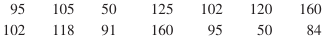
\includegraphics[width=3in]{coaster-data.png} \pause
		
		First, sort: $50, 50, 84, 91, 95, 95, 102, 102, 105, 118, 120, 125, 160, 160$ \pause
		
		There are two middle values: 102 and 102. The median is the average of these, which is 102. \pause
		
		Our graphing calculator also finds a median of $102$.
	\end{frame}

	\begin{frame}{Mode and Modal Class}
		The \textit{mode} of an ungrouped data set is the value that occurs most often. \pause
		
		The \textit{modal class} of a grouped data set is the class with the highest frequency. \pause
		
		A data set with only one mode is said to be \textit{unimodal}. \pause
		
		A data set with two modes is said to be \textit{bimodal}. \pause
		
		A data set with more than two modes is said to be \textit{multimodal}. \pause
		
		A data set in which no value occurs more than once is said to have no mode.
	\end{frame}

	\begin{frame}{Mode and Modal Class}
		The data show the number of public libraries in a sample of eight states. Find the mode.
		
		$114, 77, 21, 101, 311, 77, 159, 382$ \pause
		
		The mode is $77$. \pause
	\end{frame}

	\begin{frame}{Mode and Modal Class}
		The data show the number of gallons of various nonalcoholic drinks Americans consume in a year. Find the modal class.
		
		\begin{tabular}{|c|c|} \hline
			Drink & Gallons \\ \hline
			Soft Drinks & 52 \\ \hline
			Water & 34 \\ \hline
			Milk & 26 \\ \hline
			Coffee & 21 \\ \hline
		\end{tabular} \pause
		
		The modal class is Soft Drinks.
	\end{frame}

	\begin{frame}{Midrange}
		The \textit{midrange} of a data set is the mean of its smallest and largest values.
		
		Mathematically, $MR = \dfrac{min + max}{2}$ \pause
		
		Graphing calculators do not compute midrange for us, but they do tell us the minimum and maximum values in the data set.
	\end{frame}

	\begin{frame}{Midrange}
		The data shows the number of paid days off workers get in a sample of various countries in the world. Find the midrange of the data.
		
		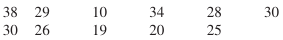
\includegraphics[width=3in]{pto-data.png} \pause
		
		$MR = \dfrac{10 + 38}{2} = 24$
	\end{frame}

	\begin{frame}{Weighted Mean}
		Sometimes, we need to find a mean where not all values are equally represented. This is called a \textit{weighted mean}. \pause
		
		For example, when computing GPA, an A is weighted more than a C. \pause
		
		The formula for computing weighted mean by hand is $\overline{X} = \dfrac{\sum (X \cdot w)}{\sum w}$ where $w$ represents the weight for the data value. \pause
		
		Graphing calculators will also compute weighted means; the method for finding a weighted mean is very similar to that for finding the mean of grouped data.
	\end{frame}

	\begin{frame}{Weighted Mean}
		A recent survey of a new diet cola reported the following percentages of people who liked the taste. Find the weighted mean of the percentages.
		
		\begin{tabular}{ccc}
			Area & \% Favored & Number Surveyed \\ \hline
			1 & 40 & 1000 \\
			2 & 30 & 3000 \\
			3 & 50 & 800
		\end{tabular} \pause
	
		The value column is \% Favored, and the weights are the Number Surveyed.
		
		By hand: $\overline{X} = \dfrac{40(1000) + 30(3000) + 50(800)}{1000 + 3000 + 800} = \dfrac{170000}{4800} \approx 35.4\%$ \pause
		
		This can be verified using a graphing calculator.
	\end{frame}

	\begin{frame}{Next Steps}
		\begin{itemize}
			\item Read 3-2
			\item Watch Video Lesson \#6
			\item Complete Assignment 3
		\end{itemize}
	
		\vfill
		
		Thanks for watching!
	\end{frame}
	
\end{document}